\documentclass[10pt]{beamer}

%%% Packages
\usepackage[ddmmyyyy]{datetime}
\usepackage[english]{babel}
\usepackage[utf8]{inputenc}
\usepackage{pythonhighlight}
\usepackage{ragged2e}
\usepackage{hyperref}

%%% Theme
\usetheme[progressbar=frametitle]{metropolis}

%%% Colors

\definecolor{blockcolor}{HTML}{FAFAFA}

%%% Configuration
\graphicspath{{img/}}

\setbeamertemplate{sections/subsections in toc}[circle]
\setbeamertemplate{enumerate items}[circle]
\apptocmd{\frame}{}{\justifying}{}

\lstnewenvironment{py}[1][]{\lstset{
    style=mypython, frame=tlrb, backgroundcolor=\color{blockcolor},
    frameround=tttt, xleftmargin=20px, xrightmargin=20px, columns=fullflexible,
    breaklines=true,
}}{}

\lstnewenvironment{bash}[1][]{\lstset{
    language=bash, frame=tlrb, backgroundcolor=\color{blockcolor},
    frameround=tttt, xleftmargin=20px, xrightmargin=20px, columns=fullflexible,
    breaklines=true,
}}{}

%%%%%%%%%%%%%%%%%%%%%%%%%%%%%%%%%%%%%%%%%%%%%%%%%%%%%%%%%%%%%%%%%%%%%%%%%%%%
%%%%%%%%%%%%%%%%%%BEGIN CONTENT OF THE PRESENTATION%%%%%%%%%%%%%%%%%%%%%%%%%
%%%%%%%%%%%%%%%%%%%%%%%%%%%%%%%%%%%%%%%%%%%%%%%%%%%%%%%%%%%%%%%%%%%%%%%%%%%%

\title[Intro to NLP]{Natual Language Processing}
\author{Alessia Mondolo}
\institute{Academy AI}
\date{August 13, 2019}
\titlegraphic{
\includegraphics[width=.10\textwidth]{logo}}

\begin{document}

\begin{frame}
  \titlepage
\end{frame}


\section{Introduction to NLP}

\begin{frame}[containsverbatim]{Introduction}
    Natural Language Processing, usually shortened as NLP, is a branch of artificial intelligence that deals with the interaction between computers and humans using the natural language.
    
    The ultimate objective of NLP is to read, decipher, understand, and make sense of the human languages in a manner that is valuable.
    
    Most NLP techniques rely on machine learning to derive meaning from human languages.
\end{frame}

\begin{frame}[containsverbatim]{NLP applications}
    Natural Language Processing is the driving force behind the following common applications:
    \begin{itemize}
        \item \textbf{Language translation} applications such as Google Translate.
        \item \textbf{Word Processors} such as Microsoft Word and Grammarly that employ NLP to check grammatical accuracy of texts, or programs able to perform automatic summarization, plagiarism detection, document classification (e.g. anti-spamming, sentiment polarity), etc.
        \item \textbf{Interactive Voice Response} (IVR) applications used in call centers to respond to certain users’ requests.
        \item \textbf{Personal assistant} applications such as OK Google, Siri, Cortana, and Alexa.
    \end{itemize}
\end{frame}

\begin{frame}[containsverbatim]{Why is NLP difficult?}
    The rules that dictate the passing of information using natural languages are not easy for computers to understand:
    \begin{itemize}
        \item Some of these rules can be high-leveled and abstract; for example, when someone uses a sarcastic remark to pass information.
        \item On the other hand, some of these rules can be low-levelled; for example, using the character “s” to signify the plurality of items.
    \end{itemize}
    
    Comprehensively understanding the human language requires \textbf{understanding both the words and how the concepts are connected} to deliver the intended message.
    
    While humans can easily master a language, the \textbf{ambiguity} and \textbf{imprecise} characteristics of the natural languages are what make NLP difficult for machines to implement.
\end{frame}

\begin{frame}[containsverbatim]{NLP problems}
    \begin{itemize}
        \item \textbf{World-knowledge:} representing world-knowledge is mandatory for understanding natual language (AI-completeness).
        \item \textbf{Multilinguality:} different languages require different models and resources. Also, there is the problem of the use of words from other languages.
        \item \textbf{Evaluation:} how to evaluate the correctness/suitability of a translation/summary?
        \item \textbf{Variability:} different sentences can refer to one meaning (e.g.: "Where can I get a map?", "I need a map", "need map" (non standard text)).
        \item \textbf{Ambiguity:} one sentence reefers to different meanings. E.g.: Ester said about Alice: "I made her duck", possible meanings:
        \begin{itemize}
            \item I cooked waterfowl for her
            \item I cooked the waterfowl she owned
            \item I created the duck she owns
            \item I caused her to quickly lower her head or body
            \item I turned her into waterfowl
        \end{itemize}
    \end{itemize}
\end{frame}

\begin{frame}[containsverbatim]{NLP techniques}
    \textbf{Syntactic analysis} and \textbf{semantic analysis} are the main techniques used to complete Natural Language Processing tasks:
    \begin{itemize}
        \item\textbf{ Syntax:} it refers to the arrangement of words in a sentence such that they make grammatical sense. In NLP, syntactic analysis is used to \textbf{assess how the natural language aligns with the grammatical rules}.
        \item \textbf{Semantics:} it refers to the meaning that is conveyed by a text. Semantic analysis is one of the difficult aspects of Natural Language Processing that has not been fully resolved yet. It involves applying computer algorithms to \textbf{understand the meaning and interpretation of words and how sentences are structured}.
    \end{itemize}
\end{frame}

\begin{frame}[containsverbatim]{Syntax}
    Some of the most used techniques in syntax analysis are:
    \begin{itemize}
        \item \textbf{Sentence breaking:} it involves placing sentence boundaries on a large piece of text.
        \item \textbf{Word segmentation:} it involves dividing a large piece of continuous text into distinct units.
        \item \textbf{Lemmatization:} it entails reducing the various inflected forms of a word into a single form for easy analysis.
        \item \textbf{Morphological segmentation:} it involves dividing words into individual units called morphemes.
        \item \textbf{Part-of-speech tagging:} it involves identifying the part of speech for every word.
        \item \textbf{Parsing:} it involves undertaking grammatical analysis for the provided sentence.
        \item \textbf{Stemming:} it involves cutting the inflected words to their root form.
    \end{itemize}
\end{frame}

\begin{frame}[containsverbatim]{Semantics}
    Some of the most used techniques in semantic analysis are:
    \begin{itemize}
        \item \textbf{Named entity recognition (NER):} it involves determining the parts of a text that can be identified and categorized into preset groups. Examples of such groups include names of people and names of places.
        \item \textbf{Word sense disambiguation:} it involves giving meaning to a word based on the context.
        \item \textbf{Natural language generation:} it involves using databases to derive semantic intentions and convert them into human language.
    \end{itemize}
\end{frame}



\section{Syntax Analysis}

\begin{frame}[containsverbatim]{Words tokenization}
    Before a program can process natural language, we need identify the words that constitute a string of characters. This is important because the meaning of text generally depends on the relations of words in that text.
    
    By default text on a computer is represented through \textttt{string} values. These values store a sequence of characters (nowadays mostly in UTF-8 format). The first step of an NLP pipeline is therefore to split the text into smaller units corresponding to the words of the language we are considering. In the context of NLP we often refer to these units as tokens, and the process of extracting these units is called tokenization.
    
    Tokenization is considered boring by most, but it's hard to overemphasize its importance, seeing as it's the first step in a long pipeline of NLP processors, and if you get this step wrong, all further steps will suffer.
\end{frame}

\begin{frame}[containsverbatim]{Words tokenization}
    \textbf{Goal:} split plain text into basic units.
    
    \textbf{Use:} Information Retrieval (IR) tasks, text categorization, sentence splitting, language identification, text normalization, etc.
    
    Different \textbf{basic units} depending on the task:
    \begin{itemize}
        \item \textbf{Naïıve tokenizations:} split by blanks and punctuation marks occurring after alphanumeric string.
        \item \textbf{Complex tokenizations:} names, clitics ("'m", "'re", "'ve", etc.), abbreviations, collocations (sequences of words that frequently occur together, e.g. ”break a leg”, ”on the one hand”), etc.
    \end{itemize}
\end{frame}

\begin{frame}[containsverbatim]{Examples of tokenization}
    \begin{figure}
        \centering
        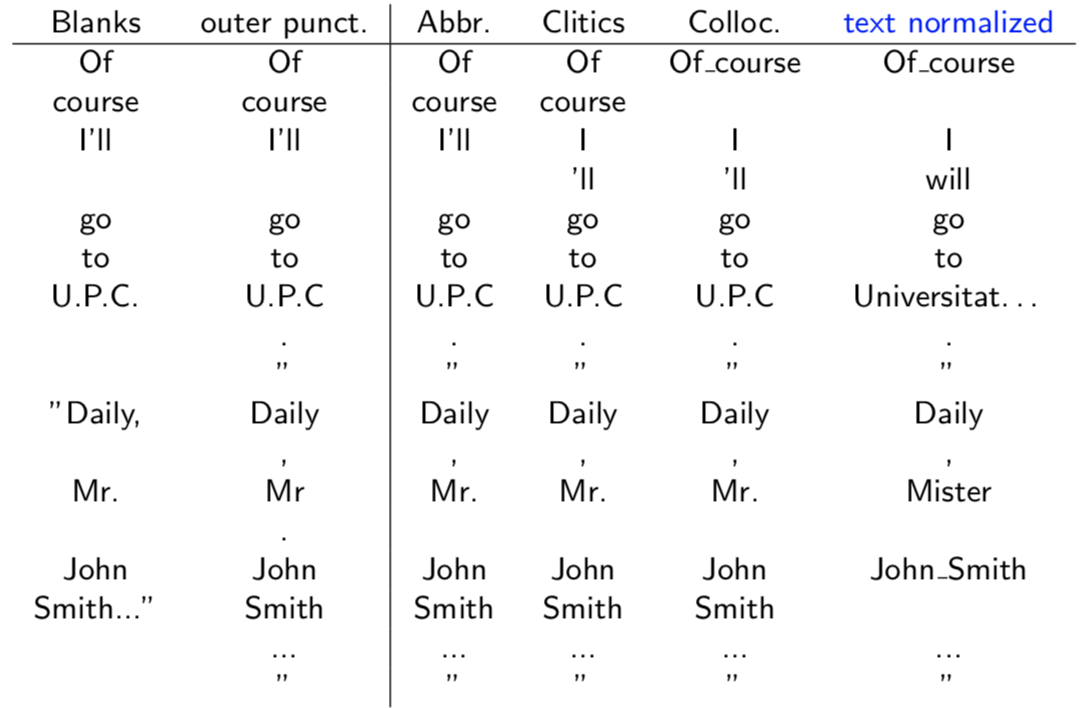
\includegraphics[width=\linewidth]{img/token.png}
    \end{figure}
\end{frame}

\begin{frame}[containsverbatim]{Sentence segmentation}
    Many NLP tools work on a sentence-by-sentence basis. The next preprocessing step is hence to segment streams of tokens into sentences. In most cases this is straightforward after tokenization, because we only need to split sentences at sentence-ending punctuation tokens.
\end{frame}

\begin{frame}[containsverbatim]{Sentence segmentation}
    \textbf{Goal:} Recognition of sentence boundaries in plain text (e.g., ’.’ ’?’ ’!’ ’...’).
    
    \textbf{Type of task:}
    \begin{itemize}
        \item Language-dependent task (e.g. German: ”Mein 2. Semester kommt bald zu Ende.”; traditional chinese?)
        \item Domain-dependent task \newline
        (e.g. ”It is expressed as (x=1)? T.add(’-’) : T.add(x).”)
    \end{itemize}
    
    \textbf{Methods:}
    \begin{itemize}
        \item Hand-crafted rules
        \item Machine learning methods
    \end{itemize}
\end{frame}

\begin{frame}[containsverbatim]{Problems of sentence segmentation}
    Main problems:
    \begin{itemize}
        \item Abbreviations and acronyms (most difficult one): "I will meet with \textbf{Mr. Smith} to talk about it.", "Lisa run \textbf{25 km. She} ended up in \textbf{N.Y.}"
        \item Ellipsis: "There’re different methods (A, B, \textbf{. . .} ) but \textbf{. . .} "
        \item Internal quotation: "'Stop!' he shouted."
        \item Ordinal numbers (German)
        \item Special cases: "We have some variables\textbf{. x} stands for the weight,"
    \end{itemize}
\end{frame}

\begin{frame}[containsverbatim]{Hand-crafted rules for sentence splitting}
    Specific hand-crafted rules for specific cases:
    \begin{itemize}
        \item Abbreviation classes (Lists of abbreviations): month name, unit-of-measure, title, address name, etc.
        \item Regular expressions for general cases, abbreviations, ellipsis, etc.:
        \begin{figure}
            \centering
            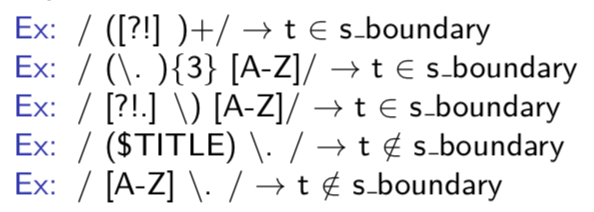
\includegraphics[width=0.6\linewidth]{img/example1.png}
        \end{figure}
    \end{itemize}
    
   \textbf{ Problem:} highly expensive adaptation to new languages (rules and abbreviation classes).
\end{frame}

\begin{frame}[containsverbatim]{Supervised ML for sentence splitting}
    \begin{itemize}
        \item The most frequently used: EM (Expectation-Maximization), SVM (support Vector Machine), CRF (Coditional Random Fields), etc.
        \item Require manually annotated corpora. Commonly,\textit{ e+,e-} = [’.’,’!’,’?’] and some preceding and following tokens
        \item Represent each \textit{e} as a set of features. Depends on the approach, the language and the domain, although normally they tend to be binary features.
        \item Problem: Require very large sets of examples (tens of thousands to hundreds of thousands)
    \end{itemize}
\end{frame}

\begin{frame}[containsverbatim]{Supervised ML for sentence splitting}
    Examples of features used in the state of the art:
    \begin{figure}
        \centering
        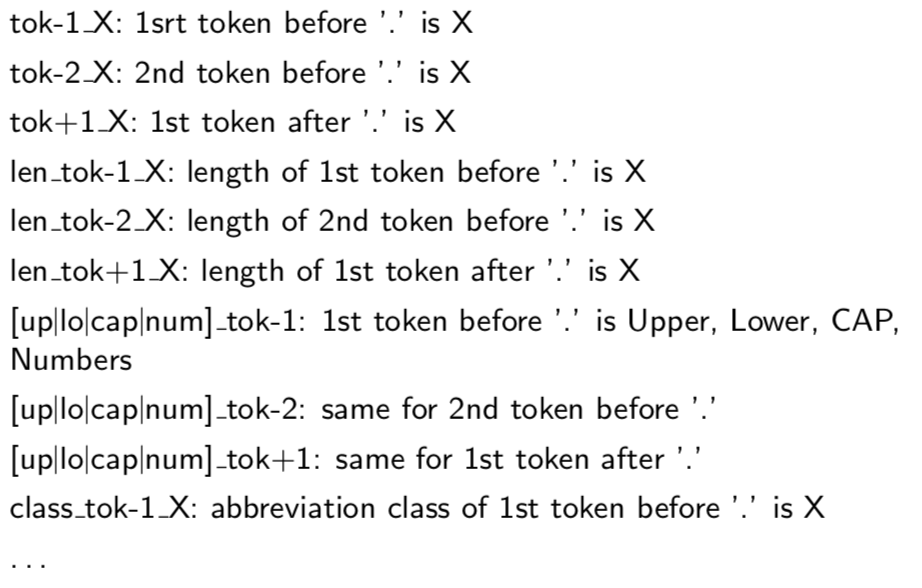
\includegraphics[width=\linewidth]{img/s1.png}
    \end{figure}
\end{frame}

\begin{frame}[containsverbatim]{Supervised ML for sentence splitting}
    Example of annotation and binary features extraction:
    \begin{figure}
        \centering
        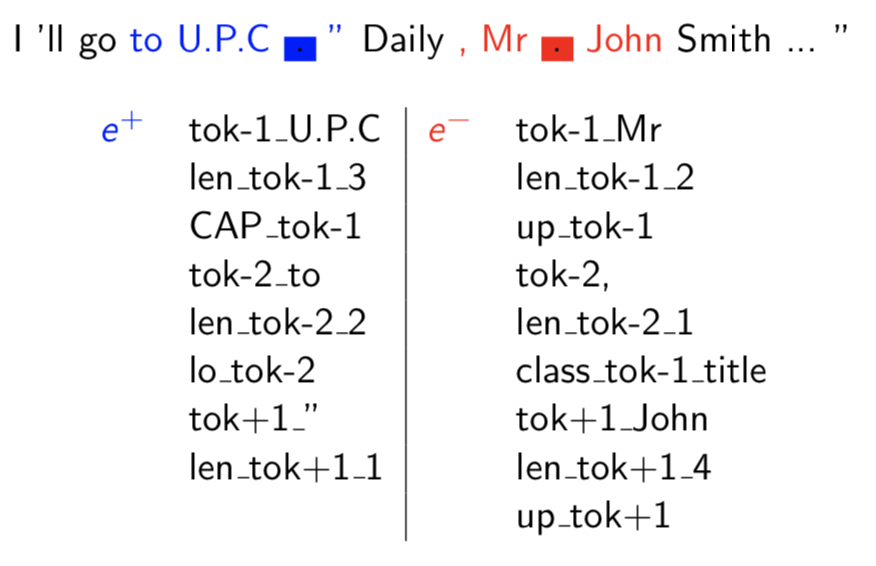
\includegraphics[width=0.9\linewidth]{img/s2.png}
    \end{figure}
\end{frame}

\begin{frame}[containsverbatim]{Unsupervised ML for sentence splitting}
    \begin{itemize}
        \item Based on corpus statistics
        \item Easily adaptable to new languages: They require large unnanotated training corpora
        \item Mainly focus on abbreviations and ellipsis
        \item Heuristics and statistics calculated from the training corpus to decide:
        \begin{enumerate}
            \item Which tokens are abbreviations?
            \item When the final period of the elements is a sentence boundary?
        \end{enumerate}
        \item Example: Punkt [Kiss and Strunk, 2006]
    \end{itemize}
\end{frame}

\section{NLTK}

\begin{frame}[containsverbatim]{NLTK}
    The Natural Language Toolkit (NLTK) is an open source Python library for Natural Language Processing.
    
    NLTK is a leading platform for building Python programs to work with human language data. It provides easy-to-use interfaces to over 50 corpora and lexical resources such as WordNet, along with a suite of text processing libraries for classification, tokenization, stemming, tagging, parsing, and semantic reasoning.
    
    \textbf{Installing NLTK:} \href{https://www.nltk.org/install.html}{link} \newline
    \textbf{Natural Language Processing with Python:} \href{https://www.nltk.org/book/}{link book}  
\end{frame}



\section{Today's homework}

\begin{frame}[containsverbatim]{Exercise}
    \begin{center}
        \href{https://colab.research.google.com/drive/1bB0Bo8RohF192g8ikRkuzW_ZQXi1kFeS}{Notebook}
    \end{center}
\end{frame}



\end{document}
